\renewcommand{\theequation}{\theenumi}
\begin{enumerate}[label=\arabic*.,ref=\thesubsubsection.\theenumi]
\numberwithin{equation}{enumi}
\item From the graph \eqref{fig:figure},
\begin{enumerate}
\item Values on X-axis represent the Bernoulli distribution of data.
\item Values on Y-axis represent the density of frequency(Histogram estimator) of the data.
\\
To calculate the histogram estimator, we have to define the number of bins(Intervals)
\\
For the graph in the question,
\begin{align}
bins=10
\\
\label{h}
h(binwidth)=\frac{\brak{1-0}}{10}
\end{align}
For bin-width h, number of observations n, for bin j, proportion of observations is
\begin{align}
p_j=\frac{y_j}{n}
\end{align}
(Where $y_j$ is the frequency of j$^th$ bin.)
\begin{align}
p_0=\frac{869}{1000}=0.869
\\
p_1=\frac{131}{1000}=0.131
\end{align}
The density estimate is
\label{understandingcurve}
\begin{align}
y\brak{x}=\frac{p_j}{h}
\\
y\brak{0}=\frac{0.869}{0.1}=8.69
\\
y\brak{0}=\frac{0.131}{0.1}=1.31
\end{align}
To draw the Gaussian Kernel Density curve,
\\
Calculate mean and standard deviation for the centre and bandwidth.
\\
See \ref{fig:fig} for clear understanding.
\begin{align}
\mu (Mean)=0.861
\\
\sigma^2 (\text{Standard Deviation})=0.1189
\end{align}
\begin{figure}[!ht]
\centering
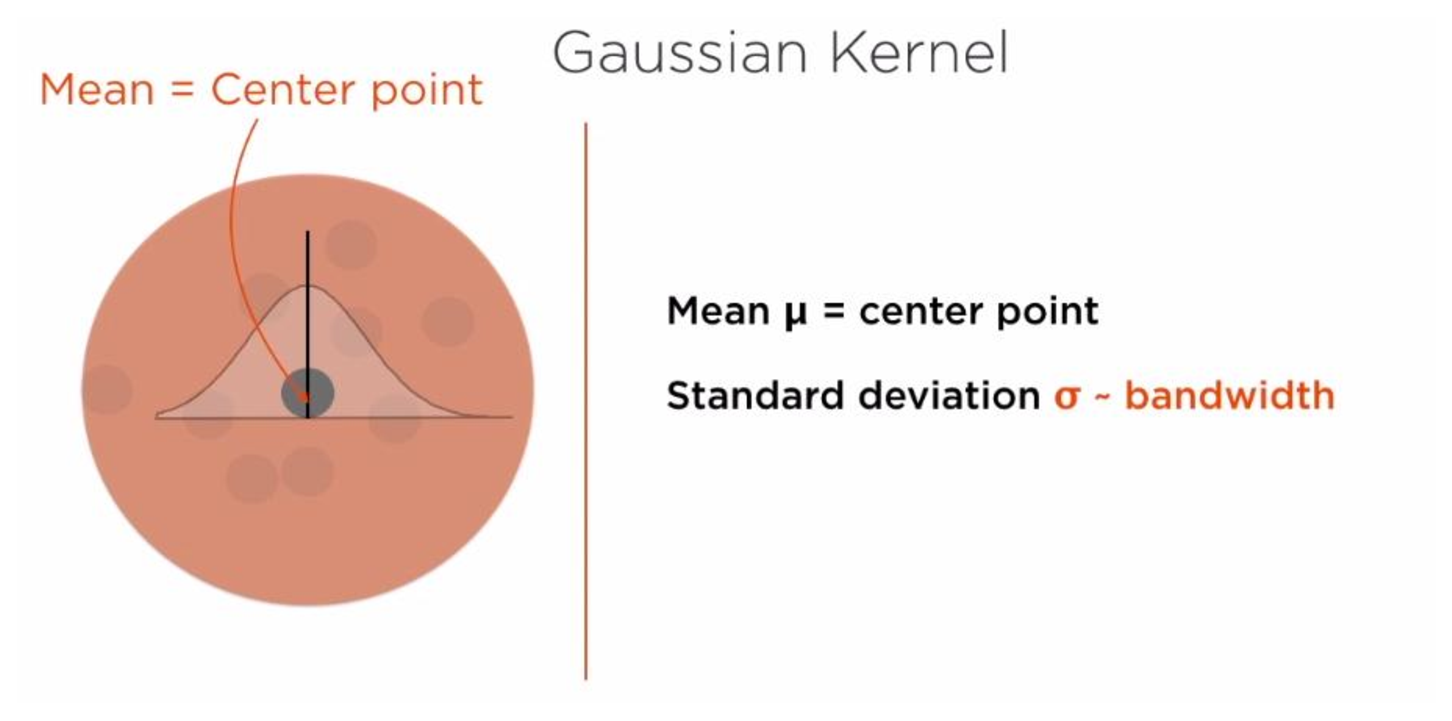
\includegraphics[width=\columnwidth]{./prob/figs/gaus_kernel.eps}
\caption{Gaussian Kernel}
\label{fig:fig}
\end{figure}

\end{enumerate}
\end{enumerate}